\documentclass[10pt,journal,compsoc]{IEEEtran}

\usepackage[utf8]{inputenc}
\usepackage{booktabs}
\usepackage{tabularx}
\usepackage{amsmath}
\usepackage{amssymb}
\usepackage{hyperref}
\usepackage{tikz}
\usepackage{colortbl}
\usepackage{xcolor}
\usepackage{pifont}
\usepackage{array}
\usepackage{multirow}
\usetikzlibrary{shapes.geometric, arrows.meta, positioning, calc, fit}

\newcommand{\cmark}{\ding{51}}
\newcommand{\xmark}{\ding{55}}
\definecolor{lightgray}{gray}{0.95}

\tikzset{
    block/.style={
        rectangle,
        rounded corners,
        draw=black,
        align=center,
        minimum width=3.5cm,
        minimum height=0.8cm,
        fill=blue!8,
        font=\small
    },
    process/.style={
        rectangle,
        draw=black,
        align=center,
        minimum width=3.5cm,
        minimum height=0.8cm,
        fill=green!8,
        font=\small
    },
    frozen/.style={
        rectangle,
        dashed,
        draw=red!80!black,
        align=center,
        minimum width=3.8cm,
        minimum height=0.85cm,
        fill=red!5,
        font=\small
    },
    loss/.style={
        diamond,
        aspect=2.4,
        draw=black,
        align=center,
        minimum width=3.2cm,
        minimum height=0.95cm,
        fill=yellow!20,
        font=\small
    },
    output/.style={
        rectangle,
        rounded corners,
        draw=black,
        align=center,
        minimum width=3.5cm,
        minimum height=0.8cm,
        fill=purple!10,
        font=\small
    },
    arrow/.style={thick, -{Stealth[scale=1.1]}}
}

\begin{document}

\title{Paper Report: Semantic-Physics Regularization for Multimodal HSI--LiDAR Classification}

\author{Benyamin Baharizadeh}

\maketitle

\begin{abstract}
This report reformulates the thesis direction as a concrete paper-oriented methodology, implementation, experimental status, and validation plan. The proposed method keeps the Cross-HL HSI--LiDAR backbone intact and adds a lightweight semantic regularization branch. A frozen CLIP text encoder is used only to build class-level semantic prototypes from physics-guided prompts. CLIP is not used as a classifier, the CLIP image encoder is not used, and hyperspectral data are not converted to RGB. The main contribution is therefore a feasible semantic-physics regularization framework for native multimodal HSI--LiDAR classification, evaluated through baseline, generic prompt, spectral prompt, and spectral+LiDAR prompt ablations. Preliminary Trento results show that the baseline is strong and that semantic regularization gives only small, setting-dependent changes in OA. Therefore, the next validation layer must include not only accuracy, but also calibration, statistical generalization, region-level behavior, boundary-region robustness, and interpretability heatmaps.
\end{abstract}

\section{Purpose of This Update}

The current work plan emphasizes three immediate tasks:

\begin{enumerate}
    \item clarify what already exists in the literature and what is different in the proposed work;
    \item formulate the contribution in a paper-oriented way, with a clear architecture and novelty statement;
    \item demonstrate technical feasibility first on HSI+LiDAR data before moving to broader generalization;
    \item add evidence that the model is interpretable, calibrated, and robust on both homogeneous regions and class boundaries.
\end{enumerate}

Accordingly, this report focuses on the current feasible implementation rather than on speculative extensions. The first experimental target remains HSI--LiDAR classification, especially Trento, followed by Houston and MUUFL for cross-dataset feasibility. Broader non-HSI modalities remain a later-stage extension.

\section{Core Research Idea}

The core idea is to investigate whether semantic priors from a frozen vision-language model can stabilize few-shot multimodal HSI--LiDAR classification.

The important design decision is that the VLM does not replace Cross-HL. The Cross-HL classifier remains the real classifier. CLIP is used only through its frozen text encoder to generate semantic class prototypes from prompts. These prototypes provide an auxiliary regularization signal during training.

\begin{quote}
\textbf{Short novelty statement:} We do not use CLIP as a classifier. We use frozen VLM text semantics as a physics-guided regularizer for the fused Cross-HL HSI+LiDAR representation.
\end{quote}

The paper story should therefore not be framed only as ``we added CLIP''. The stronger framing is that the method introduces a lightweight third semantic modality, text, into a native HSI+LiDAR classifier without replacing the classifier or forcing RGB conversion. The text modality is used as a physically meaningful prior during training, while the final decision remains produced by the task-specific multimodal model.

\section{What Is Different From Existing Work}

Many related works use foundation models through an image encoder, RGB conversion, visual prompt tuning, or large-scale remote-sensing pretraining. In contrast, the present direction preserves native HSI and LiDAR inputs and only uses the frozen text side of a VLM.

The main differences are:

\begin{itemize}
    \item \textbf{No HSI-to-RGB conversion:} HSI patches remain in native spectral form.
    \item \textbf{No CLIP image encoder:} CLIP visual features are not used.
    \item \textbf{No CLIP classification:} final predictions come from the Cross-HL classifier.
    \item \textbf{Frozen text encoder only:} CLIP text embeddings are used as semantic prototypes.
    \item \textbf{Physics-guided prompts:} prompts describe spectral material properties and LiDAR structural properties.
    \item \textbf{Backbone-preserving design:} Cross-HL remains the multimodal student backbone.
\end{itemize}

\section{Current Architecture}

Fig.~\ref{fig:current_architecture} shows the corrected architecture. The Cross-HL encoder processes native HSI and LiDAR patches. Its fused CLS feature is sent to the original classifier for cross-entropy classification. In parallel, the same fused feature is projected into CLIP text space by a small projection head and aligned with frozen text prototypes.

For the paper version, the figure should be redesigned as a polished conceptual diagram rather than a simple block workflow. The visual message should emphasize three interacting parts: native multimodal sensing, Cross-HL fusion and classification, and a frozen semantic teacher that provides physics-guided text anchors. The final figure should be redrawn manually in a paper style after using any generative tool only for visual inspiration.

\begin{figure*}[t]
    \centering
    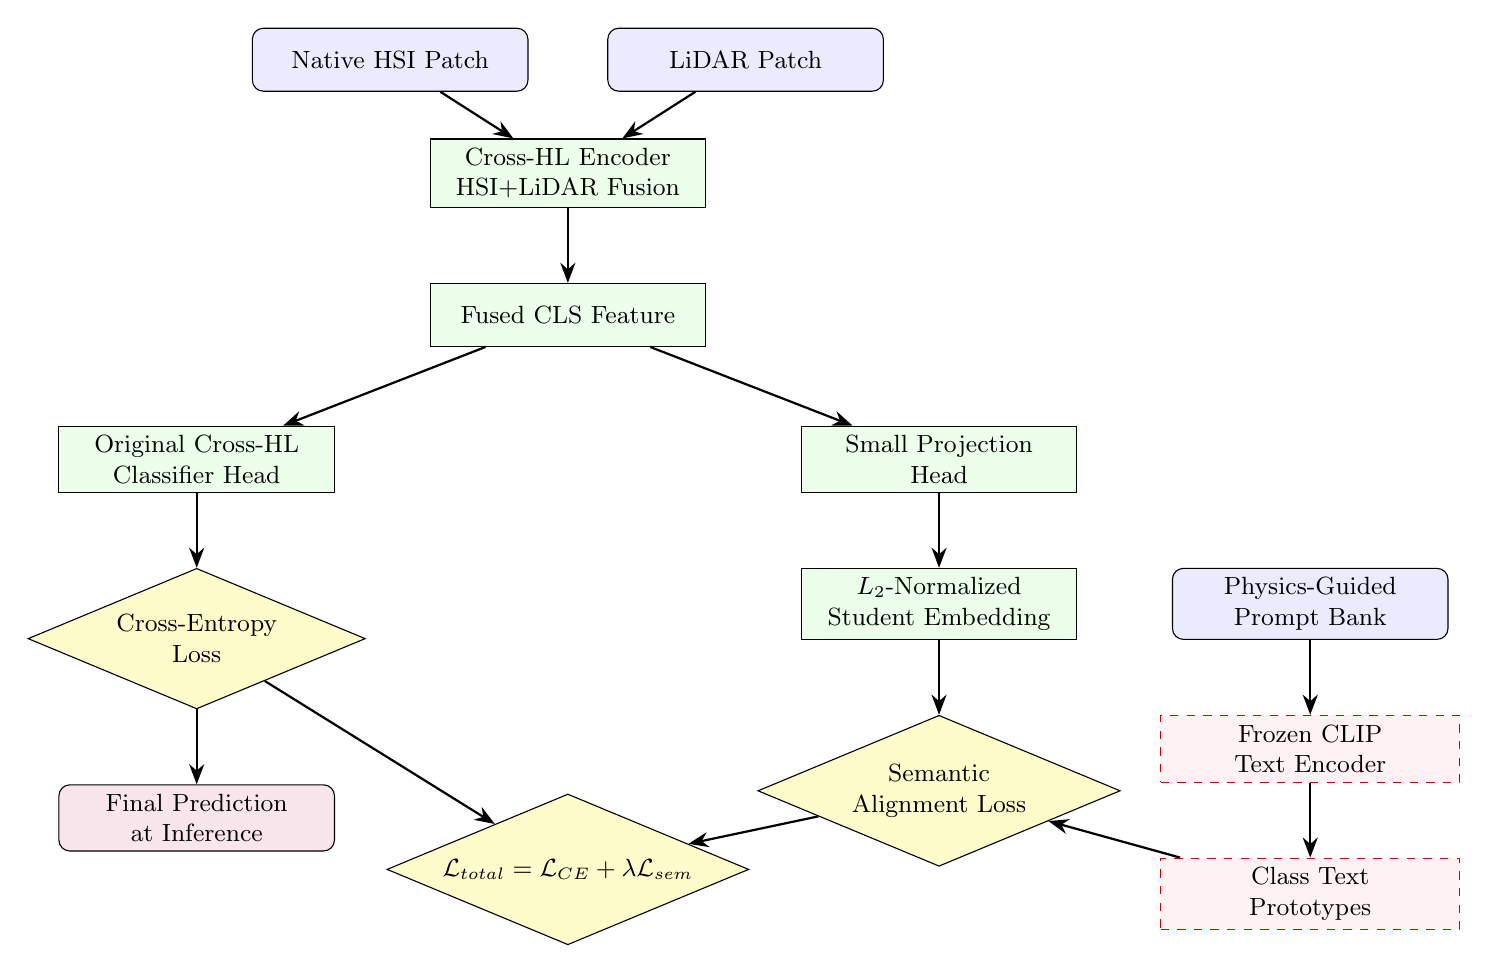
\begin{tikzpicture}[node distance=0.95cm and 1.0cm]

        \node (hsi) [block] {Native HSI Patch};
        \node (lidar) [block, right=1.0cm of hsi] {LiDAR Patch};
        \node (encoder) [process, below=1.0cm of $(hsi)!0.5!(lidar)$] {Cross-HL Encoder\\HSI+LiDAR Fusion};
        \node (feature) [process, below=of encoder] {Fused CLS Feature};

        \node (classifier) [process, below left=1.0cm and 1.2cm of feature] {Original Cross-HL\\Classifier Head};
        \node (ce) [loss, below=of classifier] {Cross-Entropy\\Loss};
        \node (pred) [output, below=of ce] {Final Prediction\\at Inference};

        \node (proj) [process, below right=1.0cm and 1.2cm of feature] {Small Projection\\Head};
        \node (embed) [process, below=of proj] {$L_2$-Normalized\\Student Embedding};
        \node (sem) [loss, below=of embed] {Semantic\\Alignment Loss};

        \node (prompts) [block, right=1.2cm of embed] {Physics-Guided\\Prompt Bank};
        \node (clip) [frozen, below=of prompts] {Frozen CLIP\\Text Encoder};
        \node (proto) [frozen, below=of clip] {Class Text\\Prototypes};

        \node (total) [loss, below=1.0cm of $(ce)!0.5!(sem)$] {$\mathcal{L}_{total}=\mathcal{L}_{CE}+\lambda\mathcal{L}_{sem}$};

        \draw [arrow] (hsi) -- (encoder);
        \draw [arrow] (lidar) -- (encoder);
        \draw [arrow] (encoder) -- (feature);
        \draw [arrow] (feature) -- (classifier);
        \draw [arrow] (classifier) -- (ce);
        \draw [arrow] (ce) -- (pred);
        \draw [arrow] (feature) -- (proj);
        \draw [arrow] (proj) -- (embed);
        \draw [arrow] (embed) -- (sem);
        \draw [arrow] (prompts) -- (clip);
        \draw [arrow] (clip) -- (proto);
        \draw [arrow] (proto) -- (sem);
        \draw [arrow] (ce) -- (total);
        \draw [arrow] (sem) -- (total);

    \end{tikzpicture}
\caption{Current CrossHL-VLM architecture. Cross-HL remains the classifier. The VLM text encoder is frozen and only supplies semantic prototypes for an auxiliary training loss. At inference, prediction is produced by the original classifier head.}
    \label{fig:current_architecture}
\end{figure*}

\section{Training Objective}

Let $x_h$ be the HSI patch, $x_l$ be the LiDAR patch, and $y$ be the ground-truth label. The Cross-HL encoder produces a fused multimodal representation:

\begin{equation}
z_s = f_{\theta}(x_h, x_l).
\end{equation}

The original classifier predicts class logits:

\begin{equation}
\hat{y} = W z_s + b.
\end{equation}

The standard classification loss is:

\begin{equation}
\mathcal{L}_{CE} = \mathrm{CrossEntropy}(\hat{y}, y).
\end{equation}

For the semantic branch, the fused feature is projected into the CLIP text embedding space:

\begin{equation}
\tilde{z}_s = \frac{g_{\phi}(z_s)}{\|g_{\phi}(z_s)\|_2},
\end{equation}

where $g_{\phi}$ is a lightweight projection head. For each class $c$, prompts are encoded by the frozen text encoder $T$:

\begin{equation}
\tilde{z}_t^c = \frac{T(p_c)}{\|T(p_c)\|_2}.
\end{equation}

The semantic alignment loss is:

\begin{equation}
\mathcal{L}_{sem} =
- \log
\frac{\exp(\tilde{z}_s \cdot \tilde{z}_t^y / \tau)}
{\sum_{c=1}^{C}\exp(\tilde{z}_s \cdot \tilde{z}_t^c / \tau)}.
\end{equation}

The total training loss is:

\begin{equation}
\mathcal{L}_{total}=\mathcal{L}_{CE}+\lambda\mathcal{L}_{sem}.
\end{equation}

The coefficient $\lambda$ is kept small so that semantic alignment acts as guidance rather than dominant supervision.

In the current implementation, an additional stabilization option is included for low-shot experiments. The semantic loss can be delayed for the first training epochs and then warmed up gradually:

\begin{equation}
\mathcal{L}_{total}(e)=\mathcal{L}_{CE}+\lambda(e)\mathcal{L}_{sem},
\end{equation}

where $\lambda(e)=0$ before the semantic start epoch and then increases linearly until it reaches the target value. This avoids forcing semantic alignment before the Cross-HL classifier has learned a basic discriminative representation. Centered text prototypes can also be used to reduce excessive cosine similarity between CLIP class prototypes.

\section{Prompt Design}

The prompt design is central to the contribution. Generic prompts are weak for HSI--LiDAR because remote-sensing classes often differ by physical characteristics rather than by visual appearance alone.

The current ablation contains three prompt settings:

\begin{itemize}
    \item \textbf{Name prompts:} generic class-name text, used as a weak semantic baseline.
    \item \textbf{Spectral prompts:} compact material and spectral descriptions, such as vegetation response, asphalt, soil, roof material, and NIR behavior.
    \item \textbf{Spectral+LiDAR prompts:} multimodal descriptions combining spectral/material properties with LiDAR geometry, such as canopy height, roof planarity, road flatness, and row structure.
\end{itemize}

Because Cross-HL learns a fused HSI+LiDAR representation, the most consistent prompt design is the spectral+LiDAR setting.

\section{Prompt Prototype Separability}

During implementation, the first physics prompts were too similar in CLIP space, especially for vegetation classes. The prompts were revised to be more class-discriminative while remaining physically meaningful.

\begin{table}[t]
\centering
\caption{CLIP text prototype similarity after prompt refinement on Trento. Lower off-diagonal similarity indicates better semantic separation between class prototypes. For Houston, centered prototypes are used when raw CLIP prototypes remain too similar.}
\label{tab:prompt_similarity}
\begin{tabular}{lcc}
\toprule
\textbf{Prompt Set} & \textbf{Mean Off-Diagonal} & \textbf{Max Off-Diagonal} \\
\midrule
Name prompts & 0.795 & 0.882 \\
Spectral prompts & 0.525 & 0.674 \\
Spectral+LiDAR prompts & 0.543 & 0.670 \\
\bottomrule
\end{tabular}
\end{table}

The refined physics prompts are substantially more separated than generic class-name prompts. This supports their use as cleaner semantic prototypes for regularization. However, prototype separation alone is not sufficient to prove improved classification performance; it should be treated as a diagnostic that explains whether the text anchors are likely to provide a useful training signal.

For datasets with many visually or semantically adjacent classes, such as Houston road, highway, railway, and parking classes, the raw CLIP text prototypes can still be highly correlated. In that case, the implementation supports class-wise prototype centering:

\begin{equation}
\bar{z}_t^c =
\frac{\tilde{z}_t^c - \frac{1}{C}\sum_{j=1}^{C}\tilde{z}_t^j}
{\left\|\tilde{z}_t^c - \frac{1}{C}\sum_{j=1}^{C}\tilde{z}_t^j\right\|_2}.
\end{equation}

This does not change CLIP or the Cross-HL backbone. It only makes the semantic anchors more discriminative before computing the alignment loss.

\begin{table}[t]
\centering
\caption{Houston prompt diagnostic for the spectral+LiDAR prompt set. Centering is used because several urban classes have highly correlated raw CLIP text prototypes.}
\label{tab:houston_centering}
\begin{tabular}{lcc}
\toprule
\textbf{Prototype Setting} & \textbf{Mean Off-Diagonal} & \textbf{Max Off-Diagonal} \\
\midrule
Raw spectral+LiDAR & 0.644 & 0.932 \\
Centered spectral+LiDAR & -0.070 & 0.734 \\
\bottomrule
\end{tabular}
\end{table}

This Houston diagnostic motivates the current code option for centered prototypes. It should be reported as an implementation stabilization step, not as a final result. Final conclusions require complete paired runs on Houston and MUUFL.

\section{Ablation Plan}

The main ablation evaluates whether semantic priors improve few-shot stability and representation separability.

\begin{table}[t]
\centering
\caption{Main ablation settings.}
\label{tab:ablation}
\begin{tabularx}{\columnwidth}{lX}
\toprule
\textbf{Setting} & \textbf{Description} \\
\midrule
Baseline & Original Cross-HL classifier only. \\
Name & Cross-HL plus semantic loss using generic class-name prompts. \\
Spectral & Cross-HL plus semantic loss using HSI spectral/material prompts. \\
Spectral+LiDAR & Cross-HL plus semantic loss using both spectral and structural LiDAR prompts. \\
\bottomrule
\end{tabularx}
\end{table}

The first completed experiments use Trento with 1\%, 5\%, and 10\% labeled data. Multiple random few-shot splits are used. All ablation methods share the same split for each iteration, giving a paired comparison against the baseline. For Houston and MUUFL, the current codebase also supports class-balanced K-shot evaluation, which is more comparable across datasets with different class sizes. A practical starting point is 20 shots per class, followed by 10 and 30 shots if time permits.

The planned metrics are:

\begin{itemize}
    \item overall accuracy (OA);
    \item average accuracy (AA);
    \item Cohen's kappa;
    \item per-class accuracy;
    \item confusion matrices;
    \item paired delta against the baseline;
    \item t-SNE of raw Cross-HL CLS features;
    \item macro-F1, micro-F1, and Matthews correlation coefficient (MCC);
    \item negative log-likelihood / log loss and expected calibration error (ECE);
    \item boundary-region and interior-region accuracy.
\end{itemize}

\section{Preliminary Results and Interpretation}

Table~\ref{tab:prelim_trento} summarizes the current Trento ablation over ten paired few-shot splits. The result should be interpreted carefully. The semantic variants are slightly above the baseline in OA and kappa at 1\%, and the spectral prompt gives a small OA improvement at 5\%. However, the effect is small relative to the split variance, AA does not consistently improve, and the 10\% baseline remains stronger than all semantic variants.

\begin{table*}[t]
\centering
\caption{Preliminary Trento ablation summary over 10 paired few-shot splits. Values are mean percentages.}
\label{tab:prelim_trento}
\begin{tabular}{lccccccccc}
\toprule
\multirow{2}{*}{\textbf{Setting}} & \multicolumn{3}{c}{\textbf{1\% labels}} & \multicolumn{3}{c}{\textbf{5\% labels}} & \multicolumn{3}{c}{\textbf{10\% labels}} \\
\cmidrule(lr){2-4}\cmidrule(lr){5-7}\cmidrule(lr){8-10}
 & \textbf{OA} & \textbf{AA} & \textbf{Kappa} & \textbf{OA} & \textbf{AA} & \textbf{Kappa} & \textbf{OA} & \textbf{AA} & \textbf{Kappa} \\
\midrule
Baseline & 83.26 & 69.03 & 77.49 & 95.31 & 90.63 & 93.71 & 96.26 & 92.58 & 94.99 \\
Name & 83.40 & 68.94 & 77.61 & 95.32 & 90.41 & 93.73 & 96.12 & 92.50 & 94.81 \\
Spectral & 83.42 & 68.95 & 77.62 & 95.33 & 90.45 & 93.75 & 96.12 & 92.52 & 94.80 \\
Spectral+LiDAR & 83.42 & 68.97 & 77.63 & 95.31 & 90.41 & 93.71 & 96.12 & 92.52 & 94.81 \\
\bottomrule
\end{tabular}
\end{table*}

The main conclusion at this stage is not that the proposed branch already beats the baseline decisively. A more accurate interpretation is that the semantic-regularization pipeline is technically feasible, but the regularization signal must be controlled carefully. The baseline is already strong, and raw CLIP text prototypes can introduce negative transfer when the semantic anchors are too similar or when the semantic loss is applied too strongly. This motivates the current low-lambda variants, delayed semantic loss, warm-up schedule, and prototype-centering option in the codebase.

For the paper narrative, this result is still valuable because it defines the real research question more sharply: under which few-shot, calibration, boundary-region, and interpretability conditions does physics-guided text regularization help a native HSI+LiDAR classifier, and when does it hurt?

\section{Generalization and Calibration Tests}

The evaluation should not rely only on OA, AA, and kappa. Reviewers may ask whether the method is better calibrated and whether it generalizes consistently across different spatial contexts. Therefore, the extended evaluation should include statistical and calibration-oriented tests:

\begin{itemize}
    \item \textbf{Macro-F1 and micro-F1:} to capture class imbalance and compare class-wise behavior.
    \item \textbf{MCC:} to provide a robust multiclass correlation score, especially when classes are imbalanced.
    \item \textbf{Log loss / negative log-likelihood:} to evaluate confidence quality, not only the final predicted label.
    \item \textbf{ECE:} to assess whether predicted probabilities are calibrated.
    \item \textbf{Paired statistical testing:} to compare baseline and semantic variants over identical few-shot splits.
\end{itemize}

This is important because semantic regularization may not always increase OA by a large margin. Its contribution may instead appear as improved calibration, reduced variance across splits, better boundary behavior, or more interpretable attention patterns.

\section{Region-Level and Boundary Evaluation}

The model should also be evaluated according to where the test patch comes from in the scene. A patch centered inside a homogeneous class region is easier than a patch centered near a class boundary, where neighboring pixels may contain mixed materials and adjacent classes. This distinction is particularly important for HSI--LiDAR scenes because roads, buildings, trees, vineyards, and bare soil often touch spatially.

The proposed additional test is:

\begin{enumerate}
    \item build a boundary mask from the ground-truth map by detecting pixels whose local neighborhood contains more than one class;
    \item define interior pixels as pixels sufficiently far from class boundaries;
    \item compute OA, AA, F1, MCC, and calibration metrics separately for boundary and interior subsets;
    \item compare whether semantic regularization helps the model remain stable near mixed-class regions.
\end{enumerate}

This analysis can support the claim that the method is not only classifying easy central regions, but also behaves reasonably in difficult edge regions where semantic and structural priors may be useful.

\section{Interpretability Plan}

The interpretability component should be grounded in actual ground-truth regions rather than only showing attractive heatmaps. The immediate goal is not to claim a full explainability method, but to provide evidence that the model focuses on physically meaningful areas when making decisions.

The proposed interpretability workflow is:

\begin{enumerate}
    \item select correctly classified and misclassified test patches from known ground-truth regions;
    \item generate heatmaps using Grad-CAM or a similar gradient-based attribution method over the HSI--LiDAR patch;
    \item overlay the heatmaps on the ground-truth class map and, where possible, on LiDAR elevation context;
    \item compare baseline and semantic-regularized models for the same patch;
    \item separately show examples from interior regions and boundary regions.
\end{enumerate}

The key question is whether the semantic-regularized model attends more consistently to the class-relevant region rather than to background or neighboring-class pixels. This connects the current VLM regularization study to the later explainability direction inspired by ShapBPT and causal evidence removal.

\section{Causal Evidence and Occlusion Extension}

A later extension can evaluate whether the model's decision truly depends on the regions highlighted by interpretability maps. The idea is to remove or mask the most important region identified by the attribution method, then re-run inference and measure the confidence drop. If the highlighted region is causally important, removing it should reduce the confidence for the predicted class more strongly than removing a random or low-attribution region.

This can be formalized as an iterative evidence-removal test:

\begin{enumerate}
    \item compute an attribution map for a correctly classified patch;
    \item mask the top-$k$ percent most important pixels or spectral-spatial elements;
    \item re-run inference and record the change in probability, logit, or loss;
    \item repeat the process iteratively to obtain an importance curve;
    \item compare baseline and semantic-regularized models.
\end{enumerate}

This direction should be presented as future work or an optional extension unless time permits. It is more ambitious than standard heatmap visualization, because it moves from explanation toward reasoning about causal visual evidence.

\section{Implementation Status}

The current implementation is feasible and modular:

\begin{itemize}
    \item the dataset loader supports Trento, Houston, and MUUFL HSI+LiDAR patches;
    \item percentage-based and class-balanced K-shot few-shot splits are implemented;
    \item the Cross-HL model is preserved and reused as the main student backbone;
    \item the VLM branch is a small projection head after the fused CLS feature;
    \item CLIP is frozen and used only for text prototype construction;
    \item prompt banks are available for name, spectral, and spectral+LiDAR settings across all three datasets;
    \item the training script writes summaries, logs, checkpoints, confusion matrices, and prompt similarity;
    \item the analysis script computes aggregate metrics, paired baseline deltas, and t-SNE plots;
    \item CUDA execution, mixed precision, TF32 acceleration, K-shot evaluation, delayed semantic loss, lambda warm-up, low-lambda variants, and centered prototypes are supported;
    \item the showcase notebook can run Trento, Houston, and MUUFL ablations from a single interface.
\end{itemize}

\section{Positioning Table for the Paper}

Table~\ref{tab:positioning} summarizes what exists, where the proposed method overlaps, and what it adds.

\begin{table*}[t]
\centering
\caption{Draft positioning against related directions. The final version should be completed after verifying the exact claims and venues of each cited paper.}
\label{tab:positioning}
\begin{tabularx}{\textwidth}{p{2.6cm}p{2.2cm}p{2.2cm}p{2.3cm}X}
\toprule
\textbf{Direction} & \textbf{Modality} & \textbf{Foundation Model Use} & \textbf{Overlap} & \textbf{Gap / Our Added Value} \\
\midrule
HSI or HSI--LiDAR deep classifiers
& HSI, LiDAR, or HSI+LiDAR
& Usually none
& Native remote-sensing classification
& Limited semantic guidance; our method adds text-based semantic regularization while preserving the classifier. \\

\midrule
Prompt tuning for HSI--LiDAR
& HSI+LiDAR
& Prompt/adaptation mechanisms
& Relevant to multimodal prompt-based learning
& Often focuses on learnable or visual prompts; our method uses frozen VLM text prototypes as semantic-physics anchors. \\

\midrule
VLM-based HSI methods
& Mostly HSI
& CLIP/VLM knowledge
& Shows language priors can help HSI
& Often uses RGB conversion, image encoders, or generic prompts; our method avoids RGB conversion and uses native HSI+LiDAR. \\

\midrule
Remote-sensing foundation models
& General remote sensing
& Large pretrained models
& Motivates foundation-model transfer
& Often requires large-scale pretraining or image encoders; our method is lightweight and text-encoder-only. \\

\midrule
Multimodal adaptation/generalization surveys
& General multimodal learning
& Foundation-model perspective
& Provides terminology and categories
& Survey-level discussion; our work instantiates a concrete HSI+LiDAR semantic-regularization pipeline. \\

\midrule
\rowcolor{lightgray}
Proposed CrossHL-VLM
& Native HSI+LiDAR
& Frozen CLIP text encoder only
& Combines multimodal fusion and language semantics
& Physics-guided spectral+LiDAR prompts regularize the fused Cross-HL representation without changing the classifier. \\
\bottomrule
\end{tabularx}
\end{table*}

\section{Dataset and Generalization Scope}

The immediate target is HSI+LiDAR. The available HSI+LiDAR datasets include Trento, Houston, and MUUFL. Therefore, the recommended sequence is:

\begin{enumerate}
    \item validate the method on Trento;
    \item if the trend is promising, extend to Houston and MUUFL;
    \item only later consider broader imaging modalities or non-HSI datasets.
\end{enumerate}

This keeps the work feasible and avoids overextending before the main methodological claim is validated.

The broader claim should be stated carefully. For a high-ambition venue, the method should eventually show that the pipeline is not limited to one HSI--LiDAR scene. The immediate feasible route is to report Trento first, then run the same protocol on Houston and MUUFL. Non-HSI medical or forensic datasets can be mentioned only as a later generalization path, not as a required result for the current thesis deadline.

\section{What to Present in the Next Meeting}

The next review should focus on progress toward a paper-ready story:

\begin{itemize}
    \item show the corrected architecture diagram;
    \item state clearly that Cross-HL remains the classifier;
    \item show the prompt similarity table;
    \item show the preliminary Trento table and state that the baseline is strong;
    \item explain that current semantic gains are small and setting-dependent, so the method needs controlled regularization rather than stronger claims;
    \item show the Houston prototype-centering diagnostic;
    \item show the ablation plan;
    \item show the extended validation plan: calibration, boundary/interior testing, and heatmaps;
    \item show the draft positioning table;
    \item report whether Houston and MUUFL K-shot runs are complete.
\end{itemize}

The recommended spoken summary is:

\begin{quote}
The current implementation makes the method concrete and feasible. The Cross-HL backbone remains intact. The model adds only a lightweight semantic branch after the fused HSI+LiDAR feature. CLIP is frozen and used only to encode physics-guided prompts into class prototypes. The first Trento results show that the baseline is already strong: semantic prompts give small improvements in the lowest-shot settings but do not consistently outperform the baseline, especially at 10\%. This means the next step is to control the semantic signal through low lambda, delayed loss, and centered prototypes, then evaluate not only OA but also calibration, boundary-region behavior, and interpretability heatmaps on ground-truth regions.
\end{quote}

\section{Expected Contribution}

The expected contribution can be stated as follows:

\begin{enumerate}
    \item a backbone-preserving semantic-physics regularization framework for native HSI--LiDAR classification;
    \item a prompt design strategy that includes both spectral/material and LiDAR structural attributes;
    \item an ablation protocol comparing baseline, generic prompts, spectral prompts, and spectral+LiDAR prompts;
    \item a paired evaluation procedure for few-shot HSI--LiDAR classification;
    \item an empirical analysis of when semantic regularization helps, when it is neutral, and when it can cause negative transfer;
    \item an extended validation protocol including calibration, boundary/interior analysis, and heatmap-based interpretability;
    \item a future path toward broader multimodal generalization and causal explainability, after validating the HSI+LiDAR case.
\end{enumerate}

\section{Next Steps}

The immediate next steps are:

\begin{enumerate}
    \item complete Houston and MUUFL K-shot ablations using centered prototypes, delayed semantic loss, and low-lambda variants;
    \item re-run or extend Trento with the stabilized semantic settings if time permits;
    \item analyze paired deltas against the baseline for all datasets;
    \item generate confusion matrices and t-SNE visualizations;
    \item add macro-F1, micro-F1, MCC, log loss, and ECE to the analysis;
    \item implement a boundary-versus-interior split from the ground-truth map;
    \item generate Grad-CAM-style heatmaps for selected ground-truth patches;
    \item complete the literature positioning table with verified papers;
    \item document negative-transfer cases clearly rather than hiding them, since they motivate the stabilization choices.
\end{enumerate}

\section{Conclusion}

The current work is now positioned as a feasible paper-oriented methodology rather than only a broad idea. The proposed CrossHL-VLM framework keeps native HSI and LiDAR processing intact, preserves the Cross-HL classification head, and uses a frozen VLM text encoder only as a semantic regularizer. The preliminary Trento results show that the baseline remains very competitive and that semantic regularization is not automatically beneficial. This is an important finding: the semantic branch must be treated as a controlled regularizer, not as a guaranteed accuracy booster. The refined prompts, prototype centering, delayed semantic loss, and low-lambda settings provide a practical route for reducing negative transfer. The immediate priority is to validate whether this semantic-physics regularization improves few-shot stability, class separability, calibration, boundary-region behavior, or interpretability indicators on Trento, Houston, and MUUFL.

\begin{thebibliography}{99}

\bibitem{cite:TeDFL}
L. Hu, W. He, L. Zhang, and H. Zhang, ``TeDFL: Toward Text-Driven Few-Shot Learning for Forest Tree Species Classification With Airborne Hyperspectral Images,'' \textit{IEEE Transactions on Geoscience and Remote Sensing}, vol. 63, 5530115, 2025.

\bibitem{cite:HZSCM}
L. Huang, Y. Chen, Z. Li, P. Ghamisi, and Q. Du, ``HZSCM: Hyperspectral Image Zero-Shot Classification via Vision-Language Models,'' \textit{IEEE Transactions on Geoscience and Remote Sensing}, vol. 63, 5528420, 2025.

\bibitem{cite:Liu2025}
Z. Liu, X. Yuan, S. Yang, G. Fu, C. Zhao, and F. Xiong, ``Multimodal Prompt Tuning for Hyperspectral and LiDAR Classification,'' \textit{Remote Sensing}, vol. 17, no. 16, 2826, 2025.

\bibitem{cite:Kong2024}
Y. Kong, Y. Cheng, Y. Chen, and X. Wang, ``Joint Classification of Hyperspectral Image and LiDAR Data Based on Spectral Prompt Tuning,'' \textit{IEEE Transactions on Geoscience and Remote Sensing}, vol. 62, 5521312, 2024.

\bibitem{cite:Dong2026}
H. Dong, M. Liu, K. Zhou, J. Kannala, C. Stachniss, E. Chatzi, and O. Fink, ``Advances in Multimodal Adaptation and Generalization: From Traditional Approaches to Foundation Models,'' \textit{IEEE Transactions on Pattern Analysis and Machine Intelligence}, vol. 48, no. 5, pp. 5672--5691, 2026.

\bibitem{cite:LDGnet}
Y. Zhang, M. Zhang, W. Li, S. Wang, and R. Tao, ``Language-Aware Domain Generalization Network for Cross-Scene Hyperspectral Image Classification,'' \textit{IEEE Transactions on Geoscience and Remote Sensing}, vol. 61, 5501312, 2023.

\bibitem{cite:ShapBPT}
M. Rashid, E. G. Amparore, E. Ferrari, and D. Verda, ``ShapBPT: Image Feature Attributions Using Data-Aware Binary Partition Trees,'' \textit{Proceedings of the AAAI Conference on Artificial Intelligence}, 2026.

\end{thebibliography}

\end{document}
